% RUL forecasting extension. Style: hyphens in compounds are fine; no em or en dashes; short captions.
The hybrid of Section~\ref{sec:method} predicts the next-cycle SOH. For deployment the
decision-relevant quantity is the remaining useful life (RUL), defined here as the number of
cycles until a cell first reaches the 0.80 end-of-life (EOL) threshold. Converting a one-step
model into an RUL forecaster is not trivial. The natural approach is to roll the model forward
autoregressively, feeding each prediction back as the next input. We find, consistent with
recent forecasting studies~\cite{seq2seq_rul, ed_lstm}, that this recursive scheme accumulates
error over the horizon and, once a cell enters nonlinear accelerated ageing, tends to
extrapolate the last observed near-linear slope and miss the knee. On the SIT cells this
failure is severe. The recursive lineage forecasts an RUL for only 38\% to 86\% of the cells
that reach EOL, and it abstains on the very cells that matter, the fast-failing G1
cells 001-8 and 101-3 that carry the manufacturing defect.

\subsection{Direct trajectory decoding}\label{sec:rul_direct}
We extend the hybrid with a direct multi-horizon decoder that predicts the whole remaining SOH
trajectory in a single forward pass, which removes the iterative feedback and its error
accumulation~\cite{seq2seq_rul, batterymformer}. The pretrained encoder, comprising the
early-life fingerprint and the observed window, is retained unchanged. A compact decoder head
outputs the SOH at a fixed set of future horizons up to 600 cycles, and the RUL is read as the
first horizon that crosses 0.80. We keep the decoder deliberately simple. On the 20-cell target
set, richer architectures overfit and lose coverage: an encoder-decoder LSTM with attention
reaches an RUL error of 96 and 43 cycles at the 30\% and 50\% anchors with coverage 79\%, and a
transformer self-attention encoder reaches 95 and 72 cycles, whereas the compact decoder reaches
68 and 49 cycles at full coverage. This is consistent with reports that simpler models dominate
when target data are scarce~\cite{cnn_robust}.

\subsection{Foundation pretraining}\label{sec:rul_foundation}
Because the target set is small, transfer is decisive. We extend the single-source pretraining
of the base hybrid into a multi-dataset LFP foundation corpus of 155 cells drawn from the MIT,
HUST, and SNL collections, and we pretrain the trajectory decoder on this corpus before
leave-one-cell-out fine-tuning on the SIT cells. This is the largest single lever we found.
Table~\ref{tab:rul} reports a clear ablation ladder. Training from scratch gives 182 and 102
cycles of error at the 30\% and 50\% anchors, MIT-only pretraining gives 85 and 100, and the
155-cell foundation corpus gives 68 and 49. Foundation pretraining also repairs calibration. The
from-scratch model is overconfident, with prediction interval coverage of 9\% to 40\%, whereas
the foundation model attains 82\% to 100\%.

\subsection{Probabilistic RUL}\label{sec:rul_prob}
We propagate the Monte Carlo Dropout ensemble through the trajectory to obtain a predictive RUL
distribution, and we report the median together with an 80\% interval calibrated by
leave-one-out conformal inference~\cite{conformal_rul}. The calibrated intervals attain 80\%
empirical coverage, and at the 50\% anchor the median width tightens from 285 to 175 cycles
relative to the raw ensemble. At the 30\% anchor the intervals remain wide, which honestly
reflects the intrinsic difficulty of forecasting a thirteenfold spread in end-of-life from
early data.

\subsection{Forecasting Accuracy and Coverage}\label{sec:rul_results}
Table~\ref{tab:rul} and Figure~\ref{fig:rul} summarise the comparison against the recursive
lineage; errors are in cycles, and a blank prediction-interval-coverage entry marks methods
that produce no intervals. The foundation model forecasts every cell that reaches EOL, including the two
catastrophic cells the recursive methods cannot, at a median error of 68 and 49 cycles and with
calibrated intervals. The recursive DE-LSTM attains a lower error, 41 and 12 cycles, but only on
the easy 38\% to 86\% of cells that it chooses to forecast. This is the coverage against risk
trade-off familiar from selective prediction~\cite{reject_option}. A method that withholds a
forecast on the defective cells is of limited use for a manufacturing screen, where those cells
are precisely the ones of interest. The direct decoder also reduces the error of the
autoregressive hybrid from 98 to 68 cycles at the earliest anchor.

\begin{table}[t]
\centering
\caption{RUL forecasting on the SIT cells.}\label{tab:rul}
\footnotesize
\setlength{\tabcolsep}{4pt}
\begin{tabular}{llccc}
\hline
Anchor & Method & Cov. & Med.\ err. & PI cov. \\
\hline
30\% & Hybrid, foundation & 100\% & 68 & 82\% \\
     & \quad abl.\ MIT only & 100\% & 85 & \\
     & \quad abl.\ from scratch & 100\% & 182 & 9 to 40\% \\
     & DE-LSTM, recursive & 38\% & 41 & \\
     & GA-LSTM, recursive & 38\% & 78 & \\
     & Hybrid, recursive & 62\% & 98 & \\
\hline
50\% & Hybrid, foundation & 100\% & 49 & 90\% \\
     & \quad abl.\ MIT only & 100\% & 100 & \\
     & DE-LSTM, recursive & 86\% & 12 & \\
     & Hybrid, recursive & 86\% & 11 & \\
\hline
\end{tabular}
\end{table}

\begin{figure*}[t]
\centering
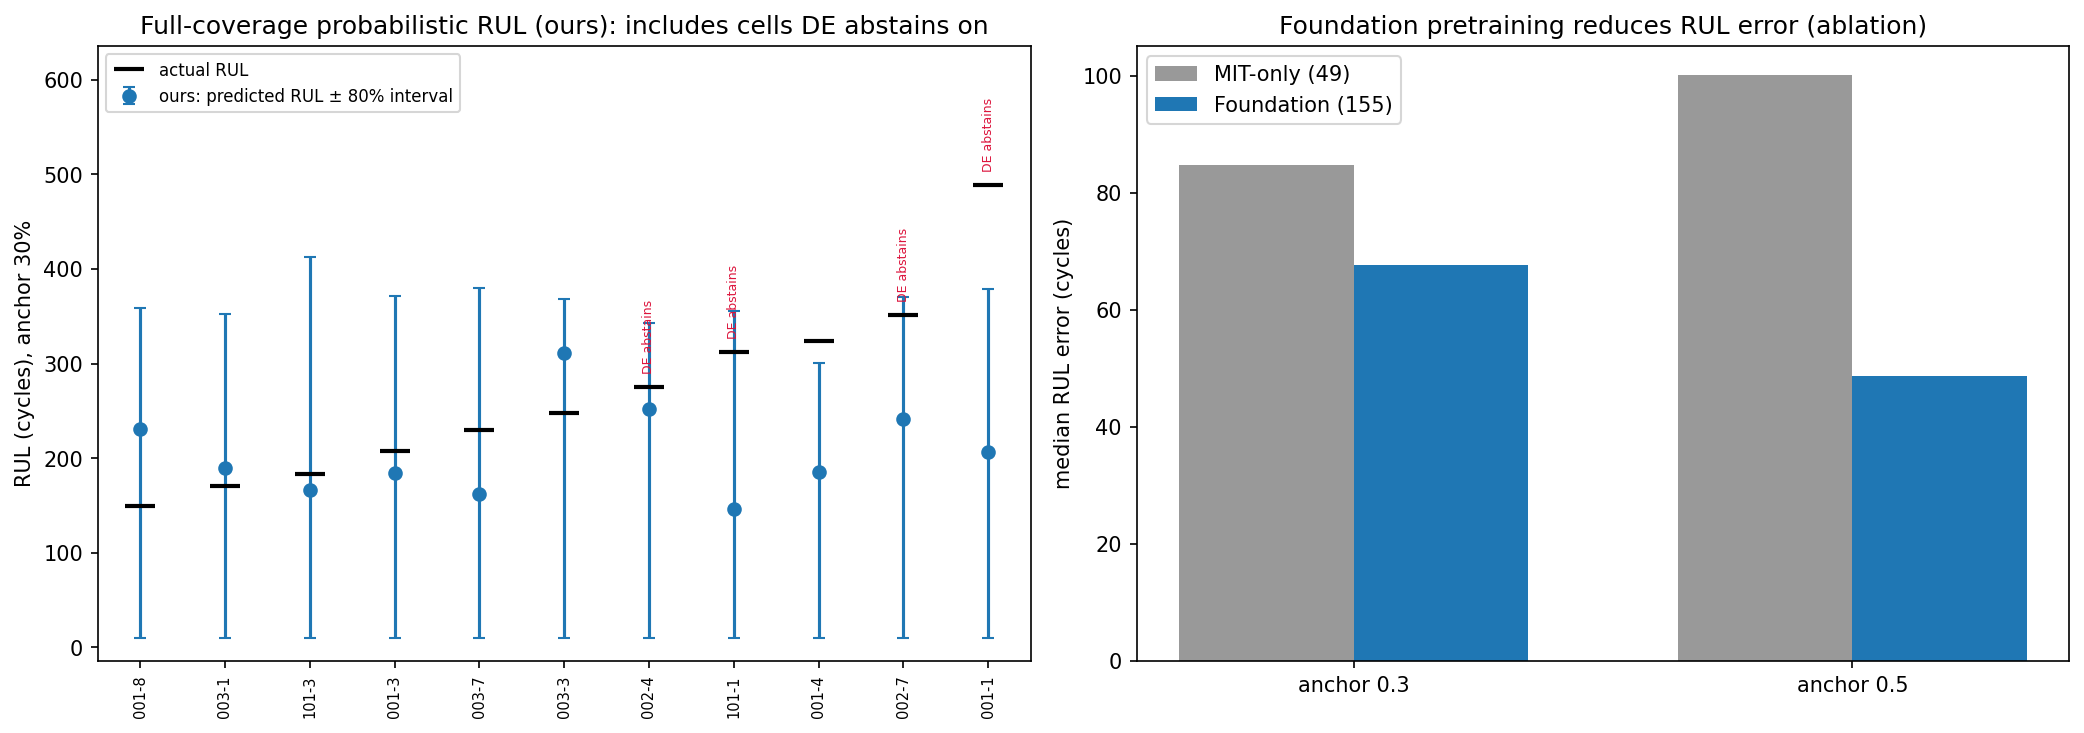
\includegraphics[width=0.9\textwidth]{figures/fig_rul_benchmark.png}
\caption{Full-coverage probabilistic RUL and the pretraining ablation.}\label{fig:rul}
\end{figure*}
